\definecolor{cobaltblue}{HTML}{0047AB}
\definecolor{techgray}{HTML}{4A4A4A}
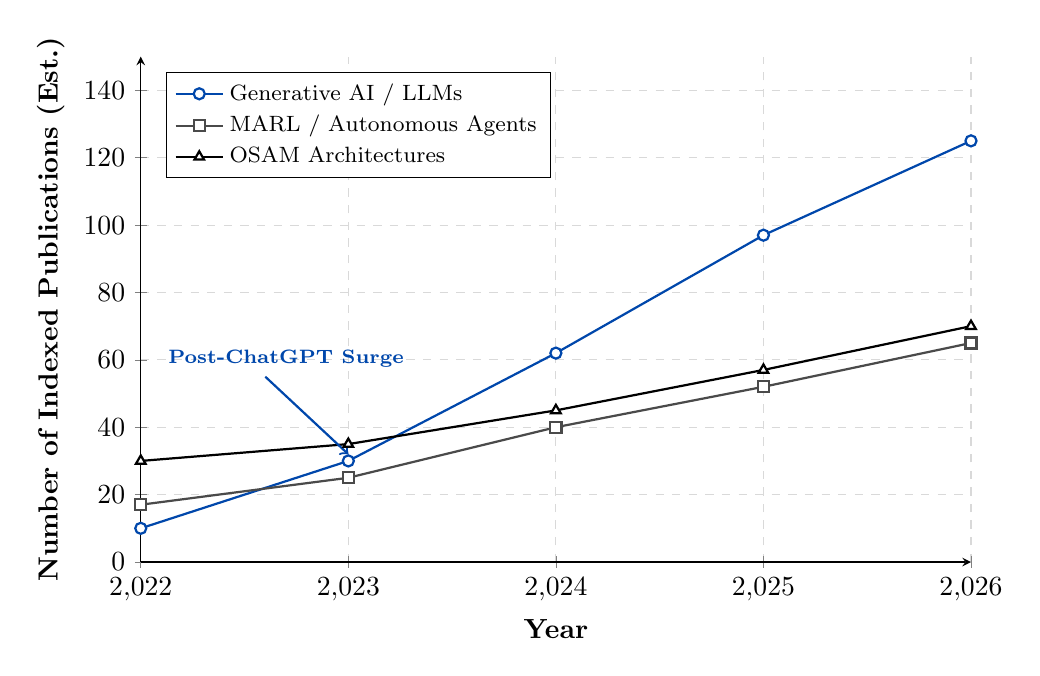
\begin{tikzpicture}
\begin{axis}[
    width=\linewidth,
    height=8cm,
    grid=major,
    grid style={dashed, gray!30},
    xlabel={\textbf{Year}},
    ylabel={\textbf{Number of Indexed Publications (Est.)}},
    xmin=2022, xmax=2026,
    ymin=0, ymax=150,
    xtick={2022, 2023, 2024, 2025, 2026},
    legend pos=north west,
    legend style={draw=black, fill=white, font=\footnotesize, cells={anchor=west}},
    axis x line=bottom,
    axis y line=left,
    clip=false % Importante para permitir anotaciones fuera del eje
]

% Serie Gen AI / LLMs
\addplot[cobaltblue, thick, mark=*, mark options={fill=white}] coordinates {(2022,10)(2023,30)(2024,62)(2025,97)(2026,125)};
\addlegendentry{Generative AI / LLMs}

% Serie MARL / Agents
\addplot[techgray, thick, mark=square*, mark options={fill=white}] coordinates {(2022,17)(2023,25)(2024,40)(2025,52)(2026,65)};
\addlegendentry{MARL / Autonomous Agents}

% Serie OSAM Archs
\addplot[black, thick, mark=triangle*, mark options={fill=white}] coordinates {(2022,30)(2023,35)(2024,45)(2025,57)(2026,70)};
\addlegendentry{OSAM Architectures}

% Anotación Post-ChatGPT Surge
\draw[->, cobaltblue, thick] (axis cs:2022.6, 55) -- (axis cs:2023, 32);
\node[cobaltblue, font=\scriptsize\bfseries, anchor=south] at (axis cs:2022.7, 55) {Post-ChatGPT Surge};

\end{axis}
\end{tikzpicture}

